\section{Parametri del sistema}
Il valore numerico di tutti i parametri d'interesse per il sistema è riportato
in \autoref{tab:parametri-numerici}. Ho misurato direttamente la maggior parte dei
parametri, esclusi quelli relativi al motore. Per
determinare questi ultimi, ho seguito il procedimento spiegato nel
paragrafo~\ref{subsec:parametri-motore}.

\bgroup
\renewcommand{\tabularxcolumn}[1]{>{\arraybackslash}m{#1}}
\renewcommand\arraystretch{1.5}
\begin{table}[H]
    \centering
\begin{tabular}{| gc | c | }
        \noalign{\hrule height 2pt}
        %todo°ò.-
        \rowcolor{Black}%
        \multicolumn{1}{=c}{\rowstyle{\bfseries\sffamily \color{White}} Parametro} & \multicolumn{1}{+c}{ Valore} \\
        \hline
        $g$ & $9,8 \sfrac m {s^2}$ \\
        \hline
        $M$ & $210g$ \\
        \hline
        $m$ & $22g$ \\
        \hline
        $l$ & $11.8cm$ \\
        \hline
        $I$ & $0.36\sfrac g {m^2}$ \\
        \hline
        $A$ & $28.5 N^{-1}$ \\
        \hline
        $B$ & $120 \sfrac s m$ \\
        \hline
        \noalign{\hrule height 2pt}
    \end{tabular}
    \caption{Parametri numerici del sistema.}
    \label{tab:parametri-numerici} %todo qui manca la descrizion2e di un tot di parametri.i
\end{table}
\egroup


\subsection{Parametri del motore}
\label{subsec:parametri-motore}
Per determinare i parametri del motore osservo il comportamento del solo
carrello quando applico un segnale $u$ costante al motore.
L'equazione che regola il comportamento del motore è la \eqref{eq:caratteristica-motore}.
L'espressione per la forza $f$
esercitata dal motore è data dalla legge di Newton
\begin{equation}
    f = M \ddot q.
    \label{eq:newton-motore}
\end{equation}
Inserisco la~\eqref{eq:newton-motore} nella~\eqref{eq:caratteristica-motore}
e applico la sostituzione
\begin{equation*}
    \left\{
    \begin{aligned}
        \dot q \mapsto v \\
        \ddot q \mapsto \dot v
    \end{aligned}
    \right.
    _.
    \label{eq:sostituzione-motore}
\end{equation*}
Ottengo
\begin{equation*}
    \dot v = \frac{u - B v} {Am}.
\end{equation*}
Fisso la condizione iniziale $v(0) = 0$ e ottengo
\begin{equation}
    v(t) = \frac u B \left(1 - e^{-\frac B {Am} t}\right).
    \label{eq:equazione-fit-motore}
\end{equation}
I parametri $A$ e $B$ sono costanti quindi, variando $u$, mi aspetto di trovare
una famiglia di curve con cui svolgere un \emph{fit} per la~\eqref{eq:equazione-fit-motore}.

In \autoref{fig:motor-vmax-fit} ho riportato i dati delle velocità in funzione di
$u$ e del tempo $t$. Chiamo $v_\infty(u)$ il limite della
curva~\eqref{eq:equazione-fit-motore} per $t \to +\infty$. I valori di
$v_\infty(u)$ sono ottenuti da una media delle velocità oltre un certo tempo.
Nella \autoref{fig:motor-vmax-fit} una linea verticale delimita i punti su cui è
stata eseguita la media e a sinistra sono riportati i valori numerici delle $v_\infty(u)$.

\begin{figure}[H]
    \centering
    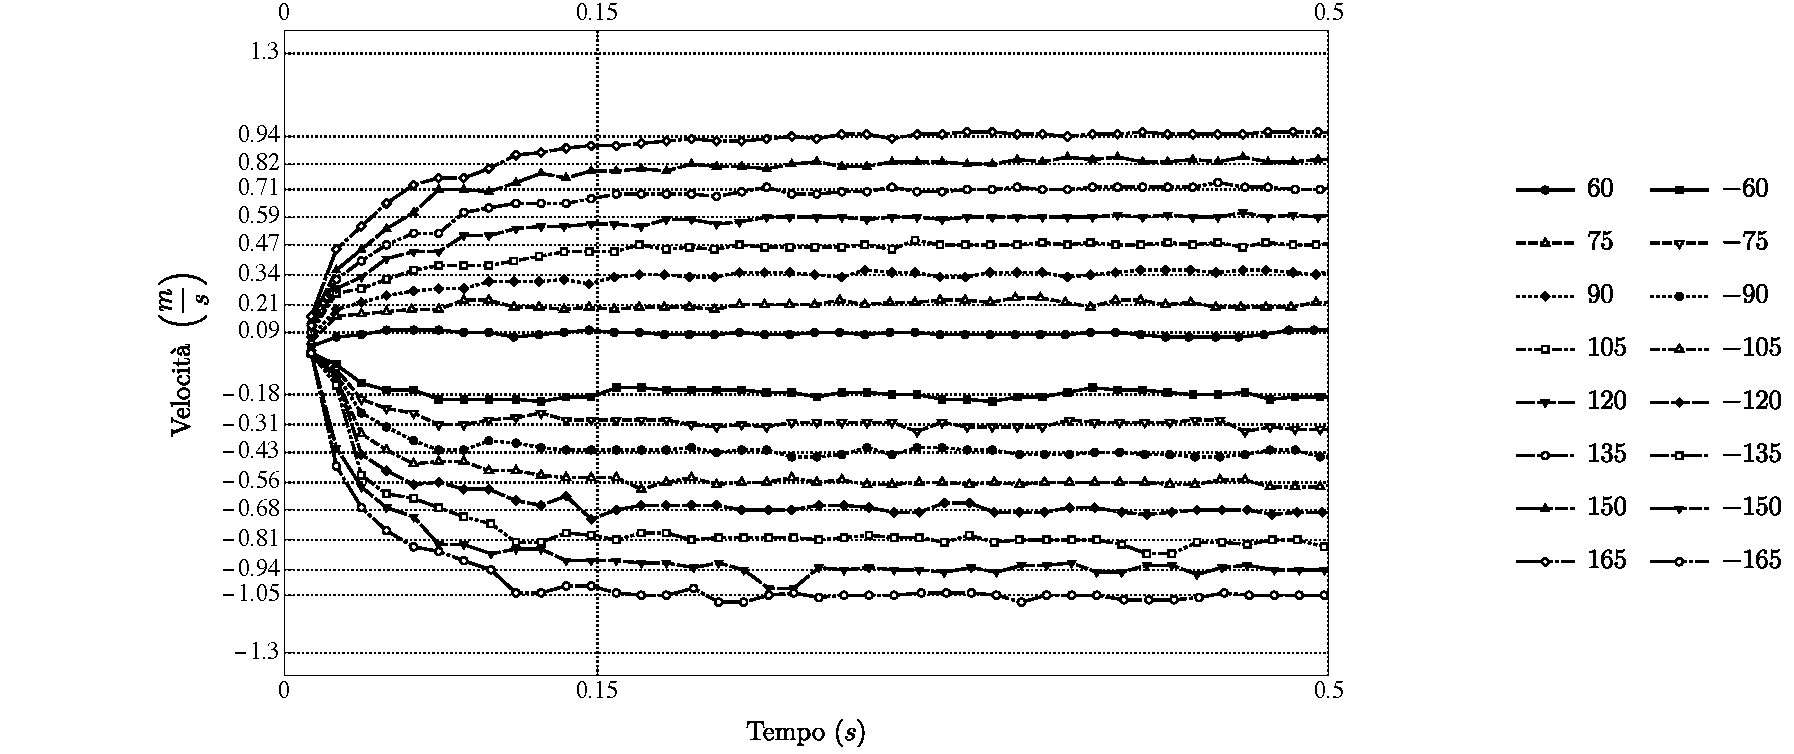
\includegraphics[width=\textwidth]{assets/motor-vmax-fit}
    \caption[Dati per stimare i parametri del motore]{Dati usati
    per stimare i parametri del motore. A sinistra sono riportati i valori
    a cui tende la velocità del carrello per un certo segnale di input al
    motore, calcolati come la media dei punti dopo il tempo $t = .15s$.
    Il valore di $u$ per ogni serie di dati è riportato in legenda, espresso
    in $(PWM)$. Vale $1 (PWM) = \sfrac {12}{255}V$.
    }
    \label{fig:motor-vmax-fit}
\end{figure}

Da un fit lineare delle $v_\infty(u)$ ricavo il parametro $B$ come inverso
della pendenza della retta
\begin{equation}
    v_\infty(u) = m u + q.
    \label{eq:vinfmuq}
\end{equation}
Il risultato del fit è riportato in \autoref{fig:motor-offset}; il valore
numerico di $B$ è
\begin{equation*}
    B = 120 \sfrac s m.
\end{equation*}

\begin{figure}[H]
    \centering
    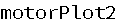
\includegraphics[width=\textwidth]{assets/motor-offset}
    \caption[Fit lineare delle velocità asintotiche del carrello]{
    Fit lineare delle $v_{\infty}(u)$. Le velocità negative e quelle positive
    giacciono su due che hanno stessa pendenza ma diversa intercetta.
    La discrepanza è dovuta all'attrito tra carrello e rotaia.
    }
    \label{fig:motor-offset}
\end{figure}

Infine ricavo $A$ da un fit esponenziale sulla famiglia di curve~\eqref{eq:equazione-fit-motore}. Il risultato è riportato in \autoref{fig:motor-expo-fit}; il valore
numerico di $A$ è
\begin{equation*}
    A = 28.5 N^{-1}.
\end{equation*}

\begin{figure}[H]
    \centering
    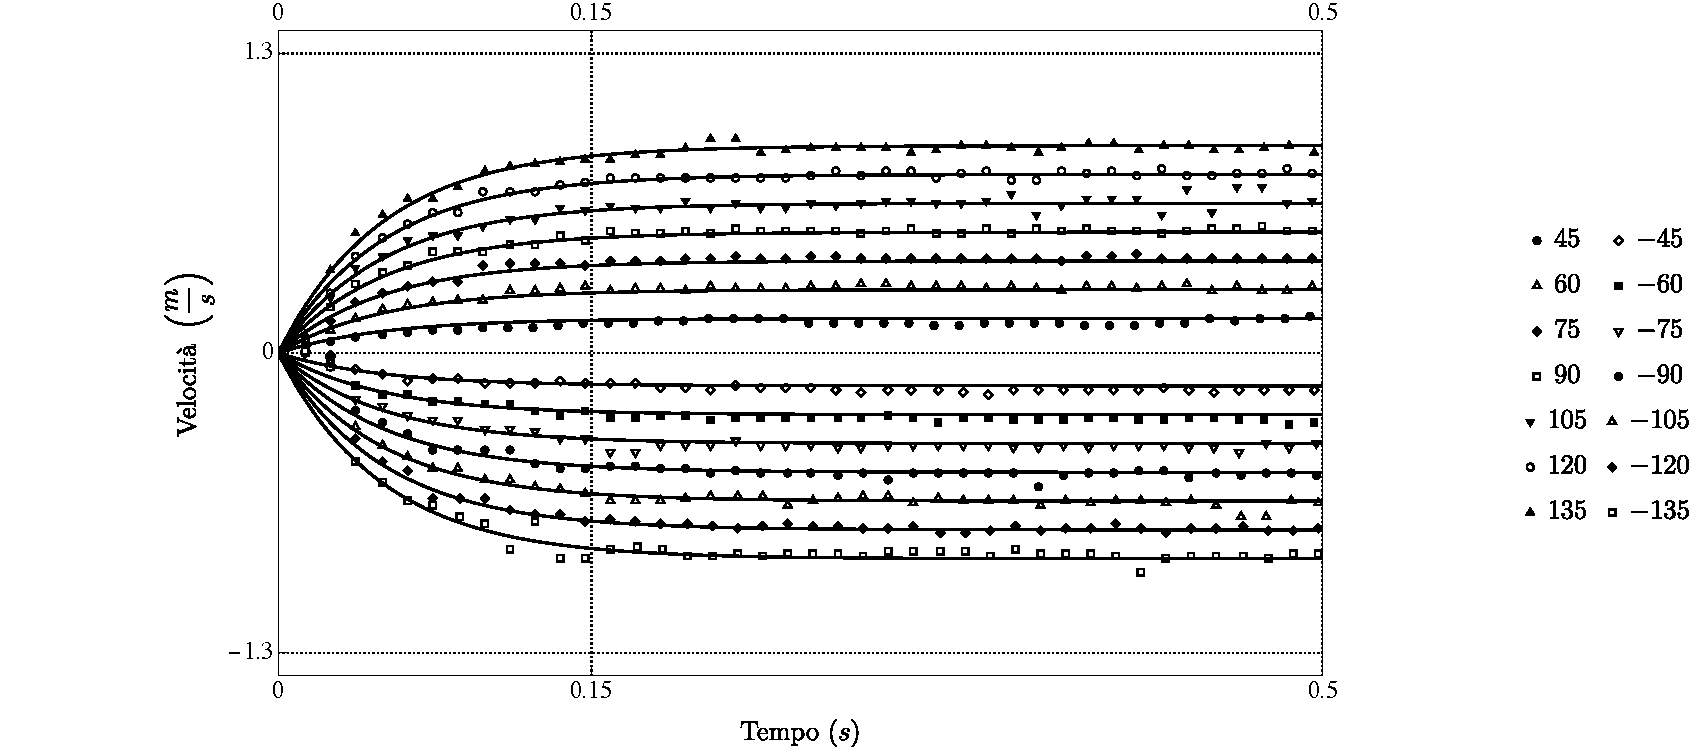
\includegraphics[width=\textwidth]{assets/motor-expo-fit}
    \caption[Fit esponenziale per i parametri del motore]{
    Fit esponenziale per trovare il parametro A del motore.
    }
    \label{fig:motor-expo-fit}
\end{figure}

Nel mio modello non compaiono attriti.
In realtà, il carrello scorre su dei cuscinetti a sfera,
quindi mi aspetto sia presente un attrito costante tra esso e la rotaia.
Fa parte degli attriti anche la \emph{coppia d'impuntamento} $\tau_c$ del motore,
dovuta all'interazione tra i magneti permanenti e le armature. $\tau_c$ ha
l'andamento descritto in \autoref{fig:cogging} ed è predominante quando $\omega$ è
piccola.
Correggo entrambi gli attriti aggiungendo un offset $u_{\min} $ a $u$, dato dall'intercetta della~\eqref{eq:vinfmuq}.

 
%fixme i have no idea what this does but i used it so that the figure next doesn't span across
%the whole page.
%\makeatletter
%\setlength{\@fptop}{0pt}
%\makeatother

\begin{figure}[H]
    \centering
    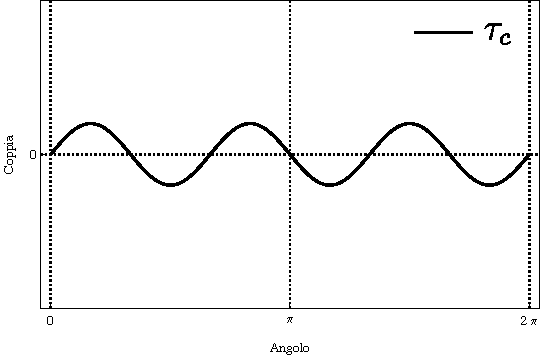
\includegraphics{assets/cogging-torque}
    \caption[Coppia d'impuntamento]{Andamento qualitativo della coppia d'impuntamento
    di un motore DC, in funzione dell'angolo del perno centrale.}
    \label{fig:cogging}
\end{figure}
